\chapter{Related Work}

\section{Standard methods for shape detection}
Before looking at the use of neural networks for shape recognition in images, some more standard approaches are presented.

\subsection{Shape detection using the Hough Transform}
Shape detection and feature extraction in images, using Hough Transforms has been a subject of research for many years. The algorithm was first popularized in computer vision in 1981 by \cite{Ballard1981} which applied a generalized version of the algorithm in order to detect of curves in gray scale images.

The article describes how boundary detection plays a crucial role for feature extraction in images, and how a generalized Hough algorithm can use edge information to define a mapping from the orientation of an edge point to a reference point related to the shape.

\subsection{Simple Linear Iterative Clustering (SLIC)}
\cite{Achanta2012} proposes a superpixel-segmentation algorithm (SLIC), which in their opinion is best suited to meet these demands. They compare their algorithm to a variety of state-of-the-art superpixel methods, and conclude that none of the existing methods are satisfactory in regards to the points.

The SLIC algorithm is fairly simple to understand. One of its key principles is that, by limiting the search space for each cluster center (points in the regular raster grid), it reduces the search speed significantly. This is achievable due to the fact that one of the primary goals of algorithm is to create a set of approximately equal sized superpixels. Thus, instead of searching the whole raster grid for each cluster center, the algorithm only has to search for edge pixels at a distance equal to D, as shown in \autoref{eq:distanceSuperpixel}.

\begin{equation}
	D'=\sqrt{\left(\frac{d_{c}}{m}\right)^{2} + \left(\frac{d_{s}}{S}\right)^{2}}
	\label{eq:distanceSuperpixel}
\end{equation}

In \autoref{eq:distanceSuperpixel} $d_{c}$ is the euclidean distance between two pixels in terms of color and $d_{s}$ is the pixels euclidean, spatial distance. Furthermore, $S$ is the sampling interval of the cluster centers ($S = \sqrt{N/k}$, where N is the number of pixels in the grid and k is the desired number of superpixels) and $m$ is a fixed constant based on the color diversity in the image.

Since the algorithm generates superpixels by clustering pixels based on their color and spatial proximity, creating a 5 dimensional, \textit{labxy} space, one would think that the distance could be found by simply taking the 5D euclidean distance. However, it turns out that for large superpixels, spatial distance outweigh the color proximity. Which is why the two distances $d_{c}$ and $d_{s}$ are weighted.

\section{The development of Convolutional neural networks}
Since McCulloch and Pitts created what is acknowledged as the first neural network in 1943, using simple electrical circuits \citep{Mcculloch1990}, they have played an important role in the field of pattern recognition. 

Since the late 1990's the idea of using convolutional operations in these networks has been considered more and more prominent \citep{LeC}, and this approach is still one of the leading research fields within ANN research \citep{Wu2017}. This section will discuss the development of the convolutional neural networks the last two decades.

\subsection{Early adaption of convolutional neural networks}
The earliest attempts of using convolutional operations for pattern and object recognition in neural networks was first done nearly twenty years ago. 

MORE HERE (LeNet)

\subsection{Deep Convolutional Neural Networks}
It was however, not until Alex Krizhevsky, Geoffrey Hinton, and Ilya Sutskever won the ImageNet \footnote{ImageNet is a very large dataset consisting of 15 million labeled, high-resolution images divided into over 22.000 categories.} 2012 competition (ILSVRC'12), that CNNs became acknowledged as one of the most sophisticated approaches for image recognition. Their deep convolutional neural network (commonly called AlexNet) consisted of five convolutional layers, each followed by a pooling layer (max-pooling), and three fully-connected softmax layers \citep{Krizhevsky2012}.  In order to reduce overfitting, the network applied two different methods; Data Augmentation and Dropout layers.

Even though the AlexNet was a big break through for the convolutional neural networks, it was criticized for not presenting a good ground for understanding what was happening inside the network, thus making it hard to improve. One of the solutions to this problem are the ZF Net, which applies deconvolutional neural networks \citep{Zeiler2011} in order to map the dense feature space produced by a CNN back to its original pixel space \citep{Zeiler2014}. \autoref{fig:deconv} shown how a deconvolutional network can help visualizing the feature space of a CNN.

\begin{figure}[!h]
	\centering
	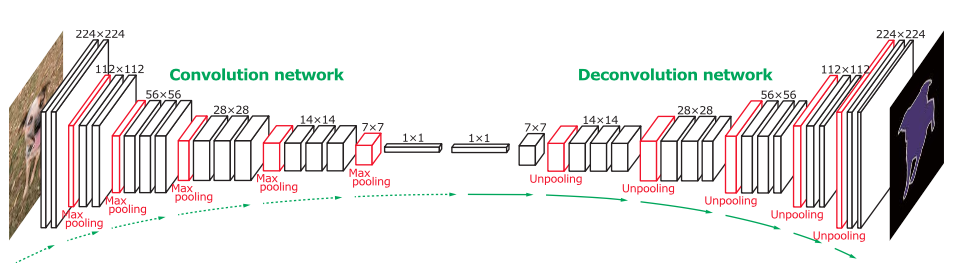
\includegraphics[scale=0.5]{fig/deconv.png}
	\caption{Process of visualizing the feature space of a CNN \citep{Noh2015}}
	\label{fig:deconv}
\end{figure}

In order to do so, the ZF Net successfully unpool, rectify and filter the feature map, generated by the CNN, in order to reconstruct the activity inside the network. 

\paragraph{Unpooling} In general, the max-pooling operation is non-reversible, since there are no tracking of the positions of the selected features, as seen in \autoref{section:pooling}. Therefore, in order to reconstruct the feature map the location of each selected maxima had to be stored.

\paragraph{Rectification}
Their CNN used the common ReLU activation function for each Convolution Layer, therefore the reconstruction layers also need to use this activation function in order to prevent negative values.

\paragraph{Filtering}
Since CNNs apply kernel filters to each convolution layers input volumes, the filtering has to be inverted when reconstructing. In order to do so, the same filters are transposed (remember that the filters are matrices) and applied to the rectified activation maps.

\subsubsection{GoogLeNet}
Another network, whose creators have criticized the standard structure of the convolutional neural networks, is the GoogLeNet \citep{Szegedy2014}. The authors of the article claims that their network was significantly more accurate than the AlexNet, while at the same time only using one twelfth of the parameters.

The GoogLeNet introduces what is called a Inception architecture (see \autoref{fig:inception} ), which main idea is to cluster neurons in the network which have highly correlated outputs. This is because in images, the correlation between pixels tend to be local. 

\begin{figure}[!h]
	\centering
	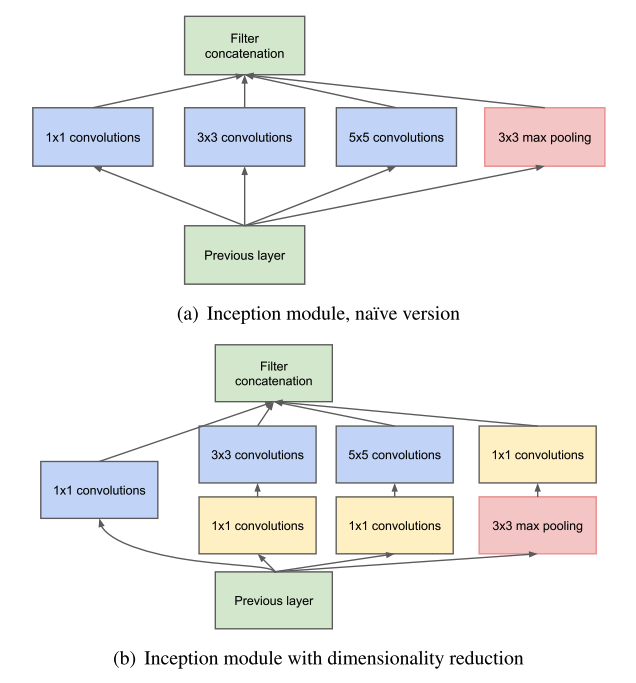
\includegraphics[scale=0.5]{fig/inception_layer.png}
	\caption{Two versions of the inception module \citep{Szegedy2014}}
	\label{fig:inception}
\end{figure}

The basic structure of the inception module is to do multiple convolution operations, in parallel, with different sized filters, and then concatenate the results before passing them on to the next layer. Additionally, a parallel pooling operation is added to each inception module, because such operations have proven them selfs successful in other CNNs.

The naive version of these "micro networks" is shown in \autoref{fig:inception} (a). One issue with this naive version is that, even with a modest number of 5x5 convolutions, the computational cost can be quite expensive. This is solved by keeping the representation of the information as sparse as possible, and only compress the signals when they have to be aggregated. In order to do so, 1x1 convolutions are used to compute reductions before the 3x3 and 5x5 convolutional operations are applied (\autoref{fig:inception} (b)).

\subsubsection{VGGNet}
Another example of a successful deep convolutional neural network is the VGGNet. This network does not present any new concepts, but the authors argue that by stacking multiple layers, doing small convolutional operations (3x3 and a few 1x1) they can outperform the other discussed networks \citep{Simonyan2014}.

\begin{figure}[!h]
	\centering
	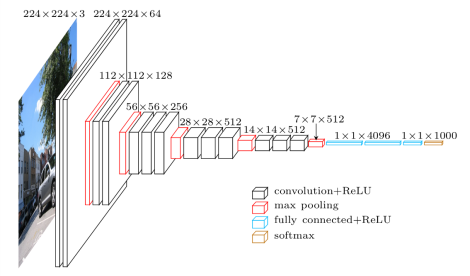
\includegraphics[scale=0.7]{fig/vgg16.png}
	\caption{The 16-layer VGGNet \citep{Frossard2016}}
	\label{fig:inception}
\end{figure}

An important difference between this network and previous networks, is that the creators focuses on depth, thus calling the network a very deep convolutional network.

\subsubsection{ResNet}
A problem that arises with deeper convolutional neural networks is the degradation problem. As depth increases in the network, the accuracy decreases (\autoref{fig:degradation}).

\begin{figure}[!h]
	\centering
	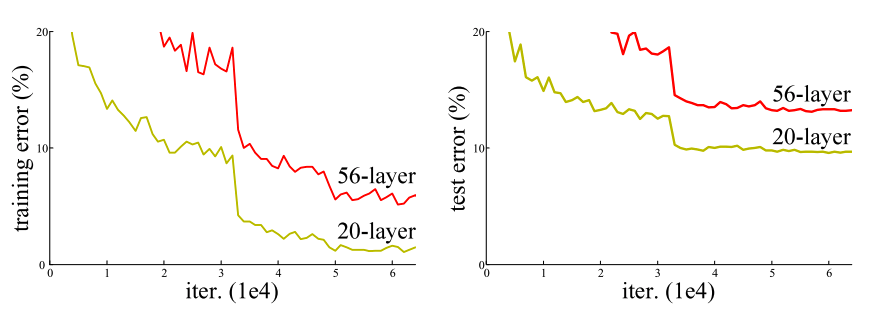
\includegraphics[scale=0.5]{fig/degradation.png}
	\caption{Degradation problem \citep{Wu2017}}
	\label{fig:degradation}
\end{figure}

Suprisingly enough this decrease in accuracy is not due to overfitting, as adding more layers effects the training error as well \citep{Wu2017}. In theory any deep network should be able to perform at least as good as a shallower network, only by seeing the layers that differenciate the two networks as identity mappings.\footnote{The map which assigns every member of a set A to the same element  $id_{A}$. It is the same as the identity function: $id(x)=x$} This however, does not seem to be the case in practice, suggesting that networks have problems learning identity mappings by multiple, non-linear layers.

In order to solve the degradation problem, the authors of the paper introduces two new concepts, which sets the foundation for their residual neural network (ResNet).

\paragraph{Residual mapping}
The paper hypothesize that it is easier to optimize residual mapping, thus introducing the residual mapping function:

\begin{equation}
	F(x) := H(x) - x
\end{equation}

where H(x) is the desired, underlying mapping function after 2 weight layers.

\paragraph{Shortcut connections}
Connections which skip one or more layers, as seen in \autoref{fig:shortcut}, in order to obtain the desired mapping function H(x).

\begin{figure}[!h]
	\centering
	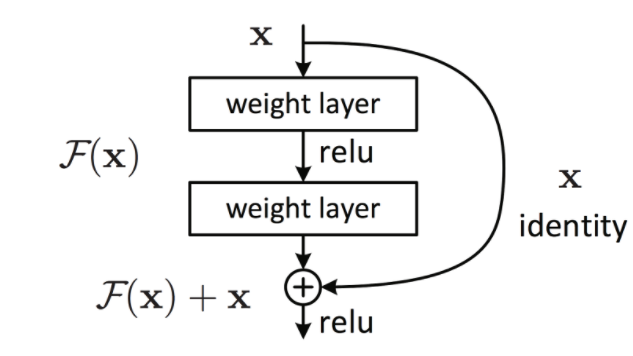
\includegraphics[scale=0.5]{fig/shortcut_connection.png}
	\caption{A residual building block \citep{Wu2017}}
	\label{fig:shortcut}
\end{figure}

Using these concepts, the authors were able to create the winning 152-layer deep ResNet of the ILSVRC'15.

Check out
http://yann.lecon.com/exdb/publis/pdf/lecun-89e.pdf

\section{Semantic segmentation using convolution neural networks}
In later years there have been a significant progress in the field of edge detection in imagery has been made due to advances in deep learning \citep{Yu2017}. Using an end to end deep semantic edge learning architecture based on ResNets \citep{Wu2017} and further extending the networks architecture with a new skip-layer, \cite{Yu2017} are able to not only identify, but also categorize edges in an image (see \autoref{fig:casenet}).

\begin{figure}[!h]
	\centering
	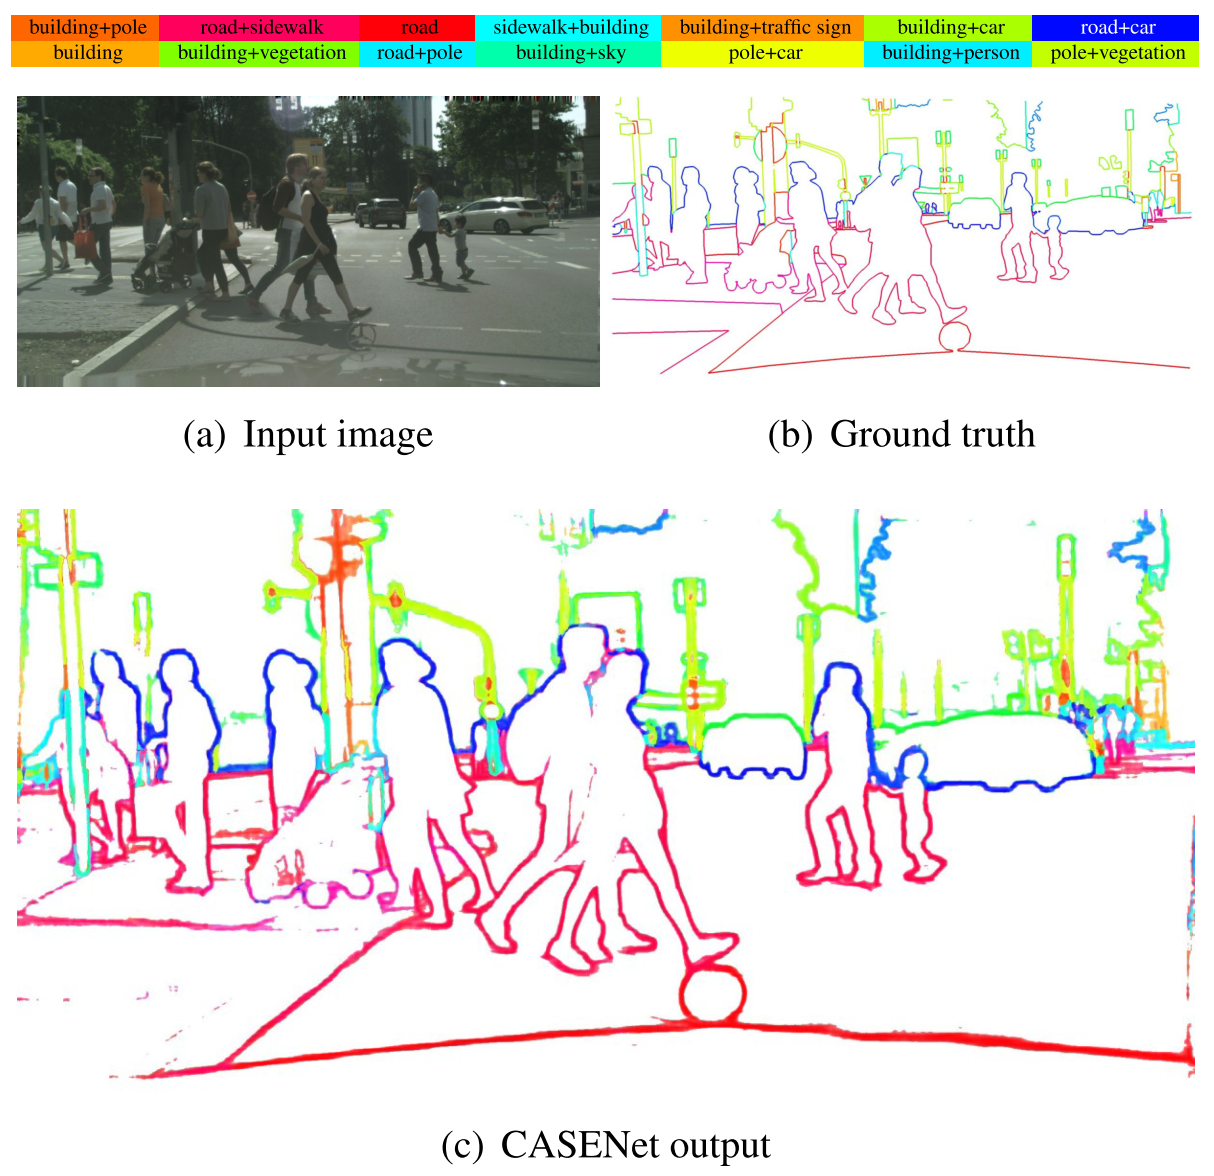
\includegraphics[scale=0.4]{fig/casenet_edge_detection.png}
	\caption{Edge detection using CASENets \citep{Yu2017}}
	\label{fig:casenet}
\end{figure}

The skip-layer uses category-wise edge activations, which are added on top of convolution layer, which share and are fused with the same set of bottom layer features. Using this approach the network produces n different edge maps, where n is the number of defined categories. Each map indicates the edge probability of e certain category.

The proposed CASENet is a modification of the ResNet-101, with some modification to the convolutional blocks, in order to preserve low-level edge information. The authors compare their network to other similar architectures, and show that their architecture outperforms state-of-the-art networks.

In terms of aerial image segmentation \cite{Kaiser2017} present a solution, which deals with the lack of labeled training data available. In order to do so, the authors make use of the open source map data library OpenStreetMap, in order to automatically derive weakly labeled training data. By matching this data with aerial imagery from Google Maps, and training a fully convolutional neural network they are able to classify buildings and roads at a high level of accuracy (see \autoref{fig:aerialsegmentation}).

\begin{figure}[!h]
	\centering
	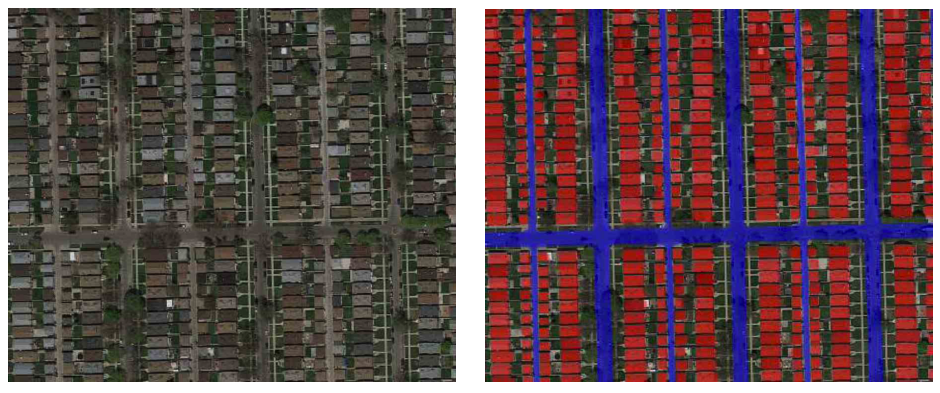
\includegraphics[scale=0.4]{fig/aerial_segmentation.png}
	\caption{Results from classification of buildings and roads \citep{Kaiser2017}}
	\label{fig:aerialsegmentation}
\end{figure}

Other attempts for semantic segmentation in remote sensing have been done with different variants of deep convolutional neural networks \citep{Kemker2017}. In their paper, they propose an approach for using the Digital Imaging and Remote Sensing Image Generation (DIRSIG) modeling software to generate a large quantity of synthetic multispectral imagery and corresponding labels. For the semantic segmentation, the authors adapt two fully-convolutional neural networks called SharpMask \citep{Pinheiro2016} and RefineNet \citep{Lin2016}. Their results show that it is possible to usesynthetic imagery can be used to assist in terms of training semantic segmentation networks when there is not enough annotated image data.

\section{Height estimation form a nadir perspective}
As seen in \autoref{section:theoreticheight} there are many different techniques that can be applied in order to estimate the height of a building. This section will focus on different attempts to retrieve height data, using satellite imagery.

\subsection{Building height retrieval from VHR SAR Imagery}
After the launch of TerraSAR-X in 2007, a satellite that was designed to acquire high-resolution X-band radar images of the entire planet, it was possible to gather SAR data with a resolution of down to 1 meter \citep{Airbus2017}. In contrast to other optical, spaceborne sensors, such as Ikonos, Quickbird and WorldView, satellites using SAR overcome the difficulties of weather conditions and lack of sun illumination.

Using the SAR images provided by the satellite \cite{Brunner2008} was able to estimate the height of man-made structures with a sub-meter precision by automatically reconstruct 3-D models, using a "hypothesis generation-rendering-matching" procedure. The basic principle was that using a optimization algorithm, the height of a building is found by testing different height hypothesis against a single SAR image. The estimation is done without modeling its exact radiometry, since this would require extensive apriori knowledge about the roughness parameters and dielectric constants of the surfaces. Generating this height model becomes an optimization problem \autoref{eq:optimizationproblem}.

\begin{equation}
	\hat{h} = arg \underset{h,\overrightarrow{s}}{max}\left\{M\left[\hat{X}_{\overrightarrow{s}}(\overrightarrow{H}),X\right]\right\}
	\label{eq:optimizationproblem}
\end{equation}

In \autoref{eq:optimizationproblem} X is the true SAR image, $\hat{X}$ is the simulated SAR image at height h, M is the matching function, and $\overrightarrow{H}$ is the simulated hypothesis.

\cite{Brunner2008} tested their method on different types of buildings, where flat buildings gave a mean accuracy of $0.3 \pm 2.1 m$. 

\subsection{Height estimation from InSAR analysis}
Another approach for height detection using SAR satellites, is interferometric SAR (InSAR) analysis, as attempted by \cite{Liu2015}. In their paper they used images taken on December 5 and 27, 2007 in order to generate an interferiogram over San Francisco. The technique was based on extracting potential layover areas from the interferiogram and use these areas to measure the height of the buildings using the relationship between the height of an object and the layover observed in the interferiogram (\autoref{eq:layoverheight}).

\begin{equation}
	\Delta\Phi=\frac{4 \pi B_{N}}{\lambda H sin{\theta}}\Delta R
	\label{eq:layoverheight}
\end{equation}

In \autoref{eq:layoverheight} $\Delta\Phi$ is the phase difference within one pixel in the layover area, $B_{N}$ is the perpendicular baseline distance, $\lambda$ is the radar wavelength, H is the satellite altitude and $\theta$ is the angle of incidence (see \autoref{fig:insar}).

\begin{figure}[!h]
	\centering
	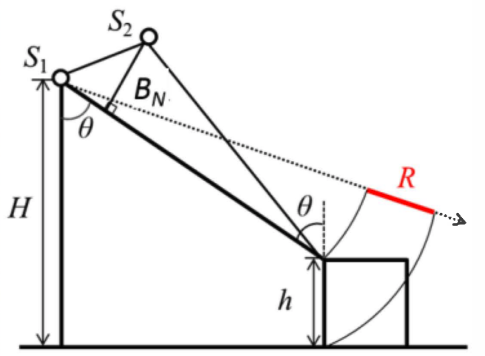
\includegraphics[scale=0.4]{fig/insar.png}
	\caption{A schematic image of geometrical characteristics for a building in a slant-range SAR image \citep{Liu2015}}
	\label{fig:insar}
\end{figure}

Using this method \cite{Liu2015} were able to estimate the height of high-rise buildings in a crowded area with a RMS of 13m and an average difference between detected results and the reference values of 6.6m.

\subsection{Height estimation using shadow measurement}
While some height extraction methods require precise specifications regarding the geometrical properties of remotely sensed data, \cite{Comber2012} present a method for determining height using building shadows. By classifying buildings and their associated shadows based on a series of different measures (see \autoref{fig:shadowclassification}), and applying \autoref{eq:shadowheight} the authors were able to give relative good height estimations.

\begin{figure}[!h]
	\centering
	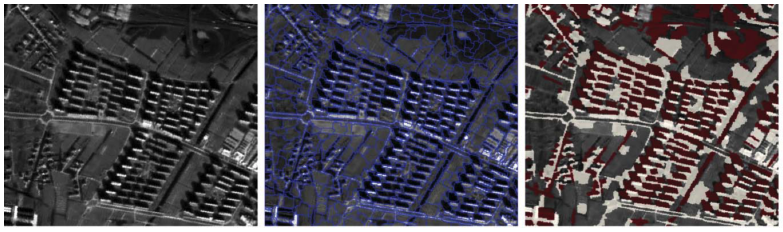
\includegraphics[scale=0.6]{fig/shadow_classification.png}
	\caption{Classification of buildings and their assiciated shadows \citep{Comber2012}}
	\label{fig:shadowclassification}
\end{figure}

\begin{equation}
	H=\frac{W}{\frac{cos(\phi_{sun}+90+\phi_{az})}{tan(\phi_{sun})}}
	\label{eq:shadowheight}
\end{equation}

Other attempts have also been made in terms of estimation heights using shadows, such as \cite{Shao2011} who addresses the issue of distinguishing between shadows and water in aerial photographs. In their approach they merged the two classes to a single shadow/water class, and used different spatial indices such as obect size, shape and spatial neighbour information in order to separate shadow and water. They further used a standard trigonometrical approach in order to estimate the building heights. Their results can be seen in \autoref{fig:shadowheightresults}.

\begin{figure}[!h]
	\centering
	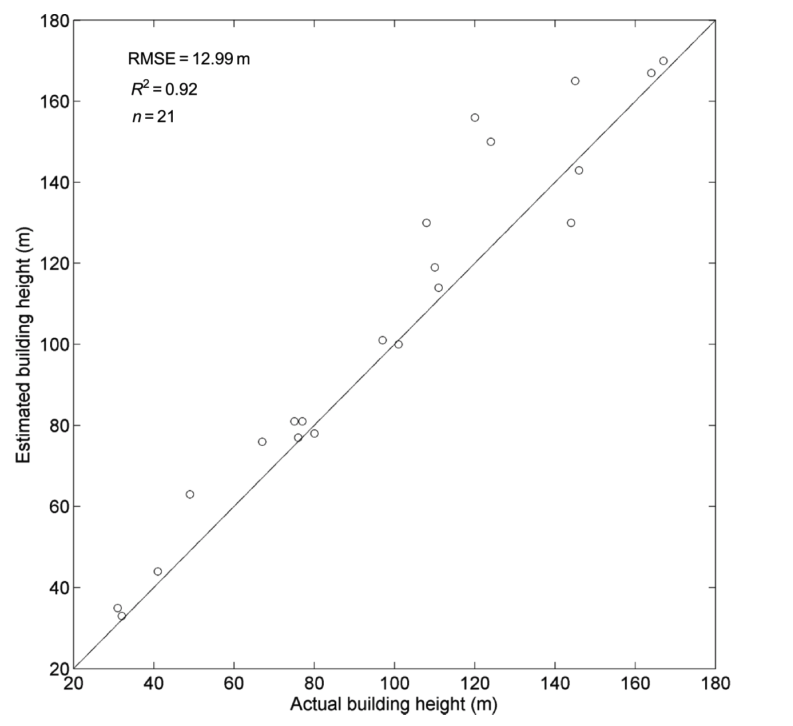
\includegraphics[scale=0.4]{fig/shadow_height_results.png}
	\caption{Accuracy evaluation of building height estimation \citep{Shao2011}}
	\label{fig:shadowheightresults}
\end{figure}